\documentclass{standalone}
\usepackage{pgfplots,pgfplotstable}
\pgfplotsset{compat=newest}
\pgfplotsset{small,legend style={font=\tiny}}

\begin{document}

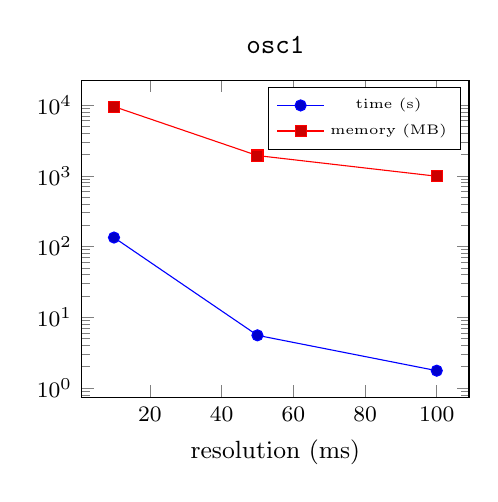
\begin{tikzpicture}
  \begin{semilogyaxis}[xlabel={resolution (ms)}, title=\texttt{osc1}]
    \addplot coordinates { (10,134) (50,5.56) (100,1.76)};
    \addplot coordinates { (10,9500) (50,1930) (100,985)};
    \legend{time (s), memory (MB)}
  \end{semilogyaxis}
\end{tikzpicture}
~
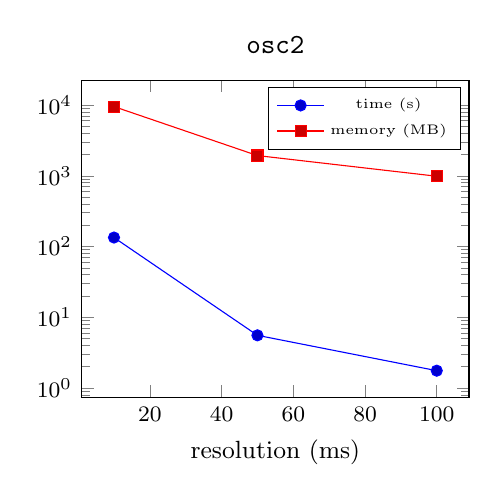
\begin{tikzpicture}
  \begin{semilogyaxis}[xlabel={resolution (ms)},title=\texttt{osc2}]
    \addplot coordinates { (10,134) (50,5.56) (100,1.76)};
    \addplot coordinates { (10,9500) (50,1930) (100,985)};
    \legend{time (s), memory (MB)}
  \end{semilogyaxis}
\end{tikzpicture}
~
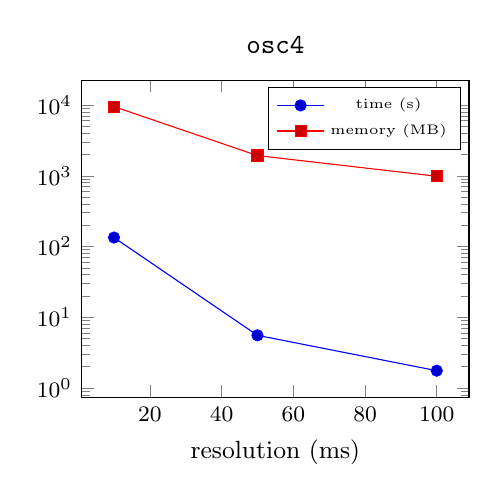
\begin{tikzpicture}
  \begin{semilogyaxis}[xlabel={resolution (ms)},title=\texttt{osc4}]
    \addplot coordinates { (10,134) (50,5.56) (100,1.76)};
    \addplot coordinates { (10,9500) (50,1930) (100,985)};
    \legend{time (s), memory (MB)}
  \end{semilogyaxis}
\end{tikzpicture}
\end{document}
